\documentclass{article}\usepackage[]{graphicx}\usepackage[]{color}
%% maxwidth is the original width if it is less than linewidth
%% otherwise use linewidth (to make sure the graphics do not exceed the margin)
\makeatletter
\def\maxwidth{ %
  \ifdim\Gin@nat@width>\linewidth
    \linewidth
  \else
    \Gin@nat@width
  \fi
}
\makeatother

\definecolor{fgcolor}{rgb}{0.345, 0.345, 0.345}
\newcommand{\hlnum}[1]{\textcolor[rgb]{0.686,0.059,0.569}{#1}}%
\newcommand{\hlstr}[1]{\textcolor[rgb]{0.192,0.494,0.8}{#1}}%
\newcommand{\hlcom}[1]{\textcolor[rgb]{0.678,0.584,0.686}{\textit{#1}}}%
\newcommand{\hlopt}[1]{\textcolor[rgb]{0,0,0}{#1}}%
\newcommand{\hlstd}[1]{\textcolor[rgb]{0.345,0.345,0.345}{#1}}%
\newcommand{\hlkwa}[1]{\textcolor[rgb]{0.161,0.373,0.58}{\textbf{#1}}}%
\newcommand{\hlkwb}[1]{\textcolor[rgb]{0.69,0.353,0.396}{#1}}%
\newcommand{\hlkwc}[1]{\textcolor[rgb]{0.333,0.667,0.333}{#1}}%
\newcommand{\hlkwd}[1]{\textcolor[rgb]{0.737,0.353,0.396}{\textbf{#1}}}%
\let\hlipl\hlkwb

\usepackage{framed}
\makeatletter
\newenvironment{kframe}{%
 \def\at@end@of@kframe{}%
 \ifinner\ifhmode%
  \def\at@end@of@kframe{\end{minipage}}%
  \begin{minipage}{\columnwidth}%
 \fi\fi%
 \def\FrameCommand##1{\hskip\@totalleftmargin \hskip-\fboxsep
 \colorbox{shadecolor}{##1}\hskip-\fboxsep
     % There is no \\@totalrightmargin, so:
     \hskip-\linewidth \hskip-\@totalleftmargin \hskip\columnwidth}%
 \MakeFramed {\advance\hsize-\width
   \@totalleftmargin\z@ \linewidth\hsize
   \@setminipage}}%
 {\par\unskip\endMakeFramed%
 \at@end@of@kframe}
\makeatother

\definecolor{shadecolor}{rgb}{.97, .97, .97}
\definecolor{messagecolor}{rgb}{0, 0, 0}
\definecolor{warningcolor}{rgb}{1, 0, 1}
\definecolor{errorcolor}{rgb}{1, 0, 0}
\newenvironment{knitrout}{}{} % an empty environment to be redefined in TeX

\usepackage{alltt}
\usepackage{graphicx}
\usepackage{microtype}
\usepackage[T1]{fontenc}
\usepackage[latin1]{inputenc}
\usepackage{lmodern}
\usepackage{geometry}
\usepackage{authblk}
\usepackage{float}
\usepackage{parskip}
\usepackage{caption}
\geometry{verbose,tmargin=2.5cm,bmargin=2.5cm,lmargin=2.5cm,rmargin=2.5cm}
\usepackage[table]{xcolor}
\bibliographystyle{unsrt}
\IfFileExists{upquote.sty}{\usepackage{upquote}}{}
\begin{document}



\title{\texttt{ASpediaFI}: Functional Interaction Analysis of AS Events}

\author[1]{Doyeong Yu}

\affil[1]{Bioinformatics Branch, Research Institute,
National Cancer Center, Gyeonggi-do, Republic of Korea}

\date{}
\maketitle
\tableofcontents
\pagebreak
%------------------------------------------------------------
\section{Introduction}
%------------------------------------------------------------
Alternative splicing (AS) is a key contributor to transcriptome and phenotypic
diversity. There are hundreds of splicing factors regulating
AS events which have a significant impact on diverse biological functions.
However, it is challenging to identify functional events related to a specific
splicing factor among thousands of them and explore their
associations with genes and pathways. We developed an R package
\texttt{ASpediaFI} for a systematic and integrative analysis of
alternative splicing events and their functional interactions.

\begin{center}
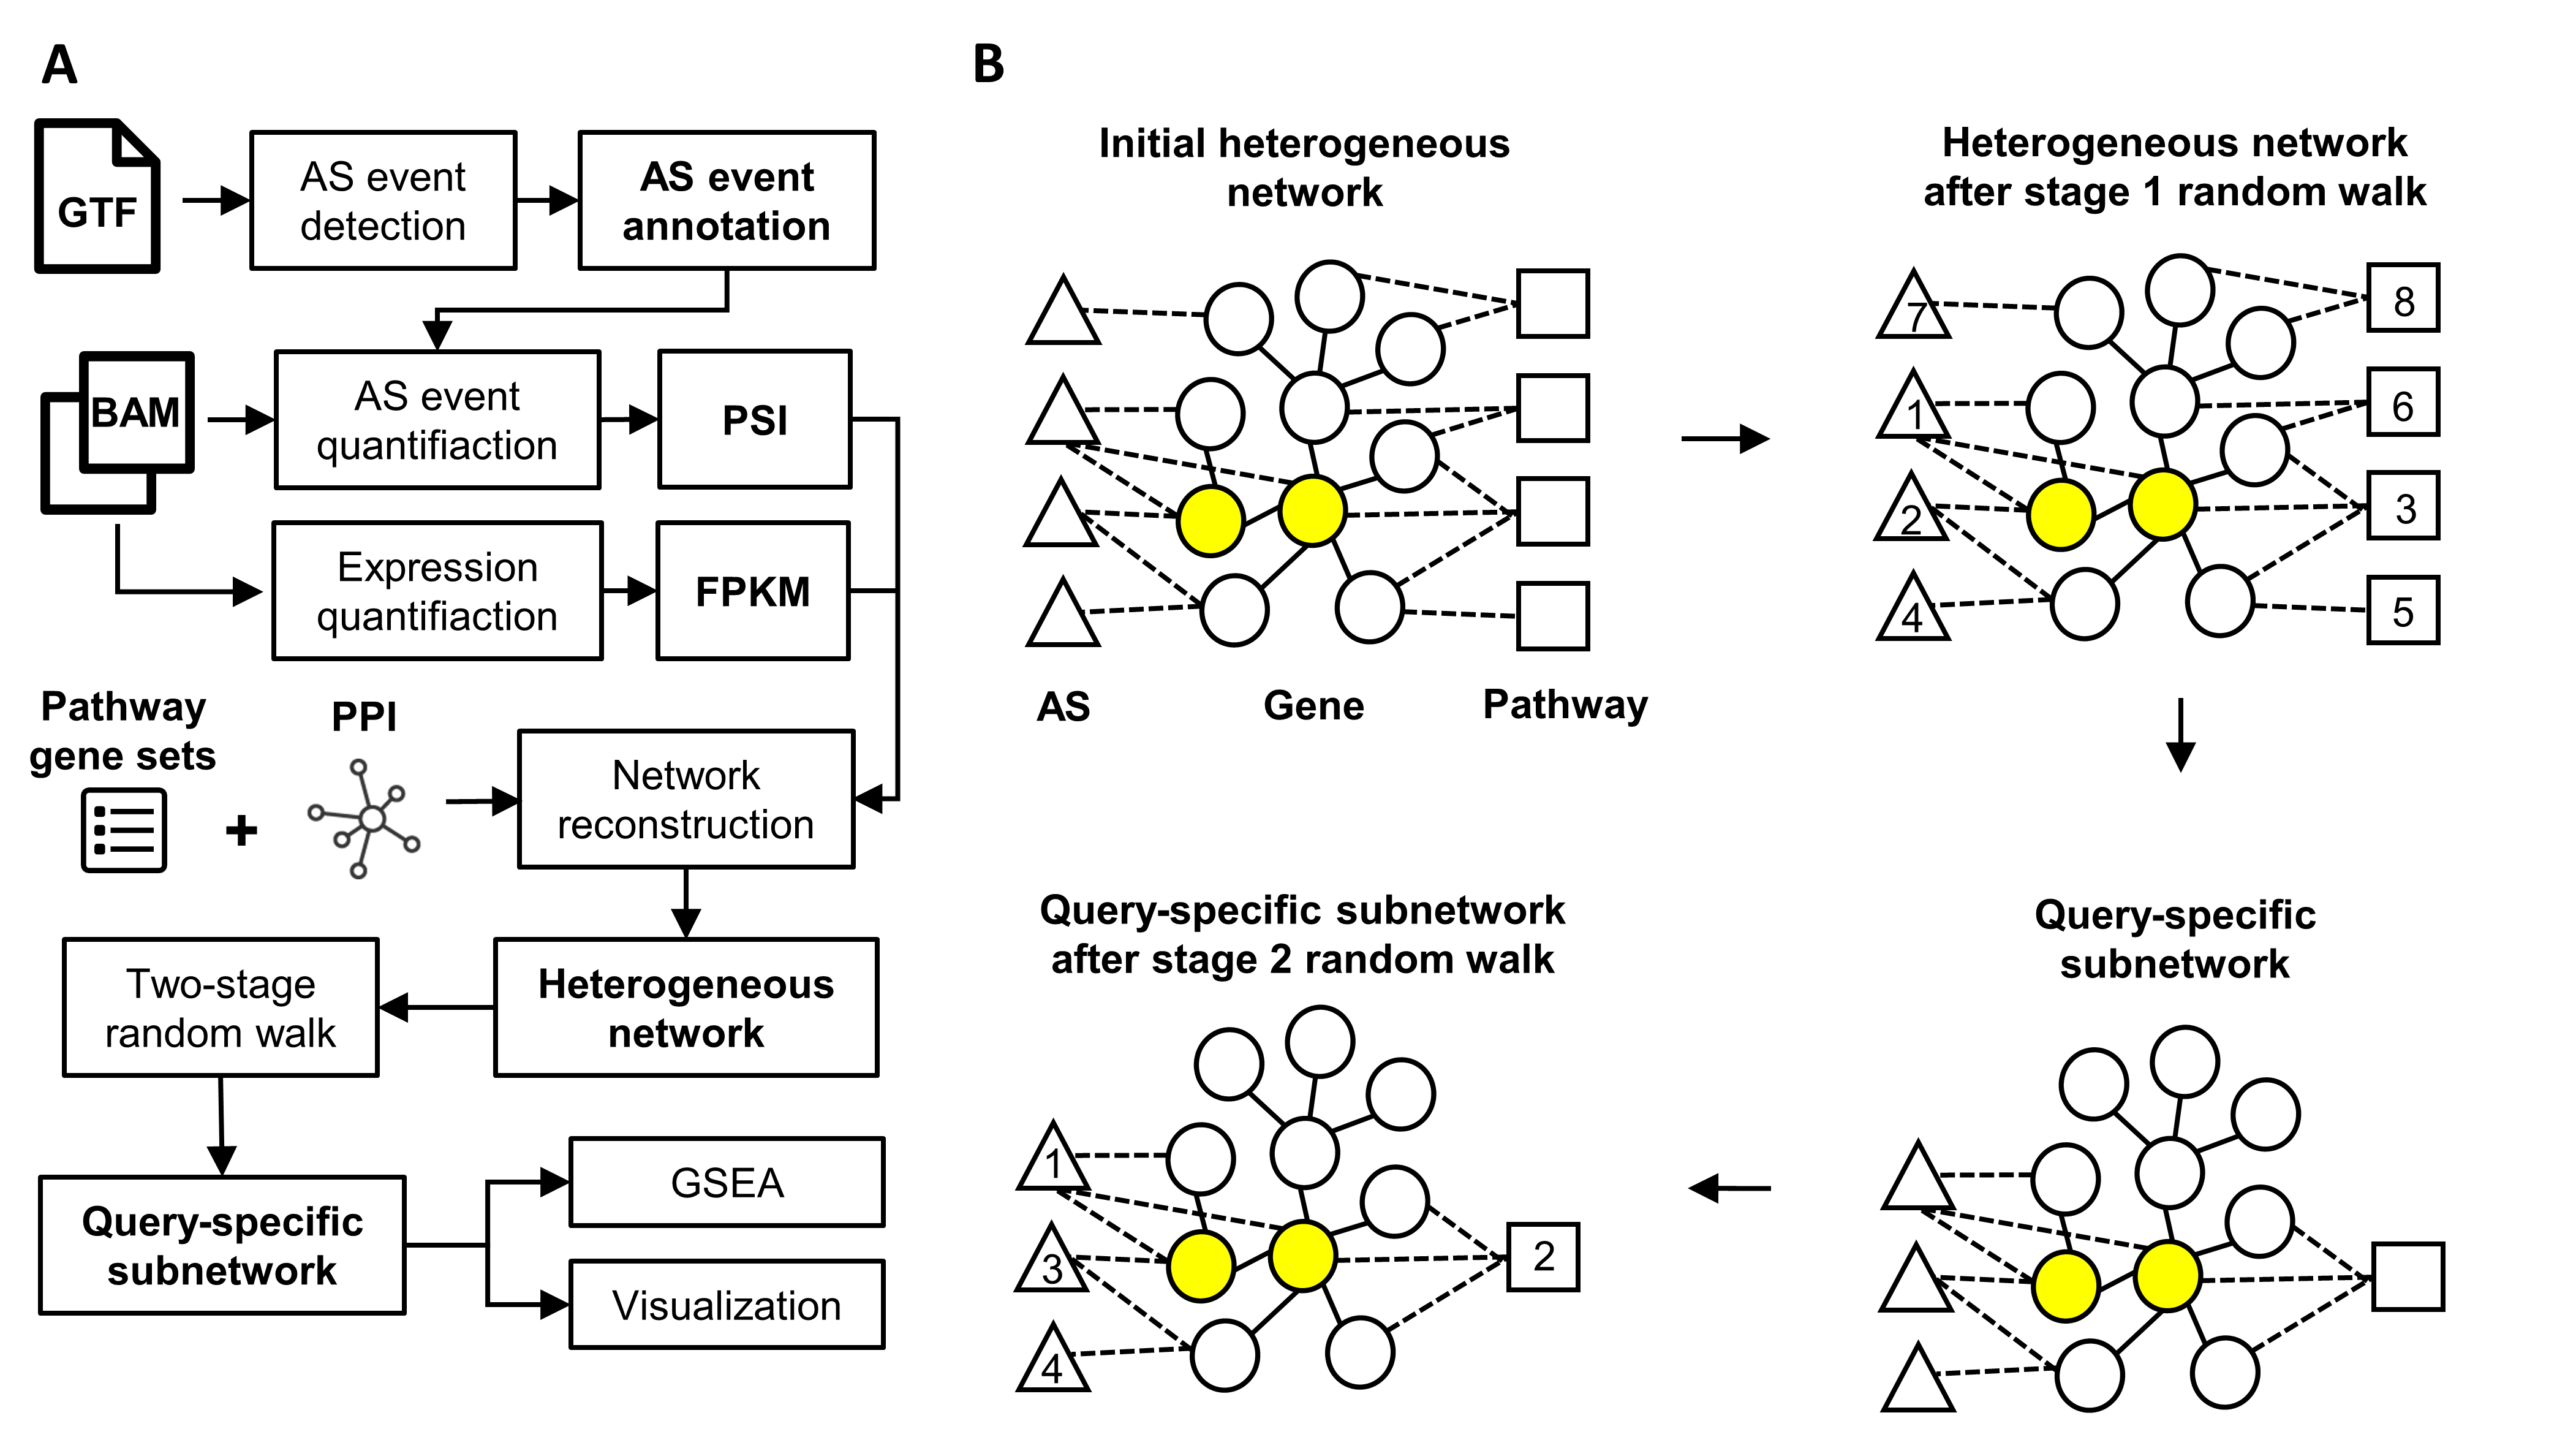
\includegraphics{Figure1.png}
\captionof{figure}{Analytic workflow of \texttt{ASpediaFI}}
\end{center}

Figure 1 shows the analytic workflow of \texttt{ASpediaFI}. The workflow
consists of the following steps:
\begin{enumerate}
\item Annotate and quantify AS events.
\item Prepare gene expression quantification, a gene-gene interaction
network, and pathway gene sets.
\item Construct a heterogeneous network comprising gene, AS event, and pathway
nodes.
\item Run DRaWR on the heterogeneous network to rank AS events and pathways
for their relevance to a splicing factor or a gene set of interest.
\end{enumerate}
At the end of the workflow, a relevant subnetwork and a ranked list of AS events
and pathways will be generated for further analysis and visualization.

%------------------------------------------------------------
\section{Installation}
%------------------------------------------------------------
To install \texttt{ASpediaFI}, enter the following commands:
\begin{knitrout}
\definecolor{shadecolor}{rgb}{0.969, 0.969, 0.969}\color{fgcolor}\begin{kframe}
\begin{alltt}
\hlkwa{if} \hlstd{(}\hlopt{!}\hlkwd{requireNamespace}\hlstd{(}\hlstr{"BiocManager"}\hlstd{,} \hlkwc{quietly} \hlstd{=} \hlnum{TRUE}\hlstd{))}
    \hlkwd{install.packages}\hlstd{(}\hlstr{"BiocManager"}\hlstd{)}
\hlstd{BiocManager}\hlopt{::}\hlkwd{install}\hlstd{(}\hlstr{"ASpediaFI"}\hlstd{)}
\end{alltt}
\end{kframe}
\end{knitrout}

\pagebreak

%------------------------------------------------------------
\section{Package contents and overview}
%------------------------------------------------------------

%------------------------------------------------------------
\subsection{Overview of \texttt{ASpediaFI}}
%------------------------------------------------------------
\texttt{ASpediaFI} provides the following functionalities:
\begin{itemize}
\item AS event detection and annotation
\item AS event quantification
\item Functional interaction analysis of AS events
\item Visualization of AS events and pathways
\end{itemize}
This package uses a reference class \texttt{ASpediaFI} as a wrapper of its
functionalities (methods) and a container of inputs and outputs
(fields).
\begin{knitrout}
\definecolor{shadecolor}{rgb}{0.969, 0.969, 0.969}\color{fgcolor}\begin{kframe}
\begin{alltt}
\hlcom{#Load the ASpediaFI package}
\hlkwd{library}\hlstd{(ASpediaFI)}

\hlcom{#Fields of the ASpediaFI reference class}
\hlstd{ASpediaFI}\hlopt{$}\hlkwd{fields}\hlstd{()}
\end{alltt}
\begin{verbatim}
               samples                 events                    psi 
          "data.frame"                 "list" "SummarizedExperiment" 
                   gtf                network             gene.table 
             "GRanges"               "igraph"           "data.frame" 
              as.table          pathway.table 
          "data.frame"           "data.frame" 
\end{verbatim}
\end{kframe}
\end{knitrout}
The \texttt{ASpediaFI} reference class contains the following fields:
\begin{itemize}
\item \texttt{samples}: a data frame containing information about samples. The
first three columns should be names, BAM file paths, and conditions.
\item \texttt{events}: a list of AS events extracted from a GTF file.
\item \texttt{psi}: a \texttt{SummarizedExperiment} object containing PSI values
of AS events.
\item \texttt{gtf}: a \texttt{GRanges} object containing genomic features
extracted from a GTF file.
\item \texttt{network}: an \texttt{igraph} object containing a query-specific
subnetwork as a result of DRaWR.
\item \texttt{gene.table}, \texttt{as.table}, \texttt{pathway.table}: data
frames containing gene nodes, AS event nodes, and pathway nodes.
\end{itemize}

\begin{knitrout}
\definecolor{shadecolor}{rgb}{0.969, 0.969, 0.969}\color{fgcolor}\begin{kframe}
\begin{alltt}
\hlcom{#Methods of the ASpediaFI reference class}
\hlkwd{setdiff}\hlstd{(ASpediaFI}\hlopt{$}\hlkwd{methods}\hlstd{(),} \hlkwd{setRefClass}\hlstd{(}\hlstr{"default"}\hlstd{)}\hlopt{$}\hlkwd{methods}\hlstd{())}
\end{alltt}
\begin{verbatim}
[1] "analyze"   "detect"    "quantify"  "visualize"
\end{verbatim}
\end{kframe}
\end{knitrout}
Other than default methods provided for all reference classes,
the \texttt{ASpediaFI} reference class includes the following methods:
\begin{itemize}
\item \texttt{detect}: detects AS events from a GTF file and save it in the
\texttt{events} field. Also extract features from a GTF file and save in the
\texttt{gtf} field.
\item \texttt{quantify}: computes PSI values of AS events from BAM files
specified in the \texttt{samples} field.
\item \texttt{analyze}: constructs a heterogeneous network of genes, AS events,
and pathways and performs DRaWR.
\item \texttt{visualize}: visualizes AS event or pathway nodes.
\end{itemize}

\pagebreak

%------------------------------------------------------------
\subsection{Case study: SF3B1 mutation in myelodysplastic syndrome}
%------------------------------------------------------------
In this vignette, we will explore all these functionalities using a
dataset of myelodysplastic syndrome (MDS) patients from the study GSE114922 [1].
This dataset contains 82 MDS patient samples, 28 of which harbored SF3B1
mutations. The RNA-Seq reads from the GEO database were aligned to the
GRCh38 genome using STAR and quantified using RSEM.

SF3B1 is one of the most frequently mutated splicing factor in MDS, and
the study have shown its association with AS events of genes involved in
heme metabolism. In the following sections, we will walk through the
\texttt{ASpediaFI} workflow shown in Figure 1 to identify AS events associated
with SF3B1 mutation and explore their functional interactions.

%------------------------------------------------------------
\section{Workflow}
%------------------------------------------------------------

%------------------------------------------------------------
\subsection{Input data preparation}
%------------------------------------------------------------
To begin, we instantiate the \texttt{ASpediaFI} class and obtain a list of
AS event annotations from a GRCh38 GTF file using the \texttt{detect} method.
Due to file size limitations, we extract AS event annotations from a subset of
GRCh38 GTF file provided in the \texttt{extdata} directory of the package.
\begin{knitrout}
\definecolor{shadecolor}{rgb}{0.969, 0.969, 0.969}\color{fgcolor}\begin{kframe}
\begin{alltt}
\hlcom{#Instantiate the ASpediaFI reference class}
\hlstd{GSE114922.ASpediaFI} \hlkwb{<-} \hlkwd{ASpediaFI}\hlstd{()}

\hlcom{#Detect and annotate AS events from a subset of the hg38 GTF file}
\hlstd{gtf} \hlkwb{<-} \hlkwd{system.file}\hlstd{(}\hlstr{"extdata/GRCh38.subset.gtf"}\hlstd{,} \hlkwc{package} \hlstd{=} \hlstr{"ASpediaFI"}\hlstd{)}
\hlstd{GSE114922.ASpediaFI}\hlopt{$}\hlkwd{detect}\hlstd{(}\hlkwc{gtf.file} \hlstd{= gtf,} \hlkwc{num.cores} \hlstd{=} \hlnum{1}\hlstd{)}
\end{alltt}
\begin{verbatim}
[1] "-------------------Processing : chr11 -------------------"
\end{verbatim}
\begin{alltt}
\hlkwd{sapply}\hlstd{(GSE114922.ASpediaFI}\hlopt{$}\hlstd{events, length)}
\end{alltt}
\begin{verbatim}
A5SS A3SS   SE  MXE   RI 
  35   21   49   40   56 
\end{verbatim}
\begin{alltt}
\hlkwd{head}\hlstd{(GSE114922.ASpediaFI}\hlopt{$}\hlstd{events}\hlopt{$}\hlstd{SE)}
\end{alltt}
\begin{verbatim}
  EnsID                Nchr    Strand 1stEX                 DownEX               
1 "ENSG00000256269.10" "chr11" "+"    "119089683-119089760" "119089217-119089272"
2 "ENSG00000256269.10" "chr11" "+"    "119089082-119089131" "119088635-119088848"
3 "ENSG00000256269.10" "chr11" "+"    "119089082-119089131" "119088635-119088707"
4 "ENSG00000256269.10" "chr11" "+"    "119089100-119089131" "119088635-119088707"
5 "ENSG00000256269.10" "chr11" "+"    "119092125-119092163" "119091413-119091526"
6 "ENSG00000256269.10" "chr11" "+"    "119092125-119092163" "119091861-119091874"
  UpEX                 
1 "119089990-119090067"
2 "119089217-119089272"
3 "119089217-119089272"
4 "119089217-119089272"
5 "119092404-119092523"
6 "119092404-119092523"
  EventID                                                                    
1 "HMBS:SE:chr11:119089217:119089272:119089683:119089760:119089990:119090067"
2 "HMBS:SE:chr11:119088635:119088848:119089082:119089131:119089217:119089272"
3 "HMBS:SE:chr11:119088635:119088707:119089082:119089131:119089217:119089272"
4 "HMBS:SE:chr11:119088635:119088707:119089100:119089131:119089217:119089272"
5 "HMBS:SE:chr11:119091413:119091526:119092125:119092163:119092404:119092523"
6 "HMBS:SE:chr11:119091861:119091874:119092125:119092163:119092404:119092523"
\end{verbatim}
\end{kframe}
\end{knitrout}
The \texttt{detect} method identifies five types of AS events:
\begin{itemize}
\item A5SS (alternative 5' splice site)
\item A3SS (alternative 3' splice site)
\item SE (skipped exon)
\item MXE (mutually exclusive exon)
\item RI (retained intron)
\end{itemize}
A list of AS event annotations contains Ensembl ID, chromosome, strand, genomic
coordinates of exons, and AS event ID. AS event ID is written in the format of
[gene symbol]:[event type]:[chromosome]:[genomic coordinates of exon boundaries]
, as defined by ASpedia. The \texttt{detect} method also extracts genomic
features from a GTF file and save in a \texttt{gtf} field as a \texttt{GRanges}
object for the visualization of AS events.

Next, we quantify AS events from BAM files using the \texttt{quantify} method.
The \texttt{quantify} method requires the \texttt{samples} field to have three
columns in the following order: name (sample ID), path (BAM file path), and
condition (sample condition). Also, a type of RNA-Seq reads (single or paired),
read length, insert size, and a minimum number of reads mapped to a given exon
need to be specified. At this point, we compute PSI values from a subset of
one BAM file for demonstration. The \texttt{quantify} method saves PSI values
in the \texttt{psi} field as a \texttt{SummarizedExperiment} object with sample
information. Note that row names of PSI values are AS event IDs.
\begin{knitrout}
\definecolor{shadecolor}{rgb}{0.969, 0.969, 0.969}\color{fgcolor}\begin{kframe}
\begin{alltt}
\hlcom{#Compute PSI values of AS events}
\hlstd{bam} \hlkwb{<-} \hlkwd{system.file}\hlstd{(}\hlstr{"extdata/GSM3167287.subset.bam"}\hlstd{,} \hlkwc{package} \hlstd{=} \hlstr{"ASpediaFI"}\hlstd{)}
\hlstd{GSE114922.ASpediaFI}\hlopt{$}\hlstd{samples} \hlkwb{<-} \hlkwd{data.frame}\hlstd{(}\hlkwc{name} \hlstd{=} \hlstr{"GSM3167287"}\hlstd{,} \hlkwc{path} \hlstd{= bam,}
                                          \hlkwc{condition} \hlstd{=} \hlstr{""}\hlstd{)}
\hlstd{GSE114922.ASpediaFI}\hlopt{$}\hlkwd{quantify}\hlstd{(}\hlkwc{read.type} \hlstd{=} \hlstr{"paired"}\hlstd{,} \hlkwc{read.length} \hlstd{=} \hlnum{100}\hlstd{,}
                             \hlkwc{insert.size} \hlstd{=} \hlnum{300}\hlstd{,} \hlkwc{min.reads} \hlstd{=} \hlnum{3}\hlstd{,} \hlkwc{num.cores} \hlstd{=} \hlnum{1}\hlstd{)}
\end{alltt}
\begin{verbatim}
[1] "Calculating PSI of SE events"
[1] "Calculating PSI of MXE events"
[1] "Calculating PSI of RI events"
[1] "Calculating PSI of ASS events"
\end{verbatim}
\begin{alltt}
\hlkwd{tail}\hlstd{(}\hlkwd{assays}\hlstd{(GSE114922.ASpediaFI}\hlopt{$}\hlstd{psi)[[}\hlnum{1}\hlstd{]])}
\end{alltt}
\begin{verbatim}
                                                      GSM3167287
HMBS:RI:chr11:119088635:119088707:119089100:119089131       1.00
HMBS:RI:chr11:119089683:119089760:119089990:119090067       0.45
HMBS:RI:chr11:119092125:119092163:119092404:119092523       0.61
HMBS:RI:chr11:119092125:119092163:119092758:119092811       1.00
HMBS:RI:chr11:119092125:119092523:119092758:119092811       0.52
HMBS:RI:chr11:119087987:119088078:119088255:119088308       0.96
\end{verbatim}
\end{kframe}
\end{knitrout}

In addition to AS event annotations and quantifications, the following are
required for network reconstruction:
\begin{itemize}
\item a named list of pathway gene sets
\item an \texttt{igraph} object containing a gene-gene interaction network
\item a matrix or \texttt{SummarizedExperiment} object containing gene
expression profiles (FPKM)
\end{itemize}
If the first two inputs are not given, \texttt{ASpediaFI} uses a combined list
of HALLMARK, KEGG, and REACTOME pathway gene sets and a network with gene
interactions collected from BIND, DIP, HPRD, and REACTOME. Gene expression
quantifications must be prepared by the user using quantification tools such as
RSEM and Cufflinks. Here, we use gene expression profiles of MDS patients
stored in the package as an example dataset. Since we need sample information
and AS event quantifications for all samples, we also load the example dataset
containing PSI values and sample information to update the \texttt{psi} and
\texttt{samples} fields.
\begin{knitrout}
\definecolor{shadecolor}{rgb}{0.969, 0.969, 0.969}\color{fgcolor}\begin{kframe}
\begin{alltt}
\hlcom{#Load PSI and gene expression data}
\hlkwd{data}\hlstd{(}\hlstr{"GSE114922.fpkm"}\hlstd{)}
\hlkwd{data}\hlstd{(}\hlstr{"GSE114922.psi"}\hlstd{)}

\hlcom{#Update the "samples" and "psi" fields}
\hlstd{GSE114922.ASpediaFI}\hlopt{$}\hlstd{psi} \hlkwb{<-} \hlstd{GSE114922.psi}
\hlstd{GSE114922.ASpediaFI}\hlopt{$}\hlstd{samples} \hlkwb{<-} \hlkwd{as.data.frame}\hlstd{(}\hlkwd{colData}\hlstd{(GSE114922.psi))}

\hlkwd{head}\hlstd{(GSE114922.ASpediaFI}\hlopt{$}\hlstd{samples)}
\end{alltt}
\begin{verbatim}
                 name path condition
GSM3167287 GSM3167287            MUT
GSM3167290 GSM3167290             WT
GSM3167294 GSM3167294            MUT
GSM3167295 GSM3167295             WT
GSM3167297 GSM3167297            MUT
GSM3167298 GSM3167298             WT
\end{verbatim}
\end{kframe}
\end{knitrout}

%------------------------------------------------------------
\subsection{Functional interaction analysis of AS events}
%------------------------------------------------------------
The \texttt{analyze} method performs data preprocessing, network construction
and DRaWR (Discriminative Random Walk with Restart) [2]. AS event and gene
expression quantifications, a gene-gene interaction network, and pathway gene
sets are  used to construct a heterogeneous network composed of gene, AS event,
and pathway nodes. DRaWR is then applied to identify AS events and pathways
associated with a gene set of interest.

The DRaWR algorithm consists of two stages of random walk with restart (RWR).
RWR is run on the heterogeneous network twice in the first stage, one with
a query gene set and another with all genes as the restart set. AS events and
pathways are ranked by the difference between the converged probability
distributions in two times of RWR. In the second stage, RWR is run on a
subnetwork composed of all gene nodes and top \textit{k} ranked feature
(AS event or pathway) nodes to obtain final rankings of genes and features.

As the DRaWR algorithm requires a query gene set as input, we first perform
t-test on the gene expression dataset to detect genes differentially expressed
in SF3B1-mutated samples. These DEGs are used as a query to identify AS events
and pathways closely related to SF3B1 mutation. If a query is given as a
character vector, all genes in the query have equal weights. The user can
attribute distinct weights by providing a data frame containing the weights
in the second column as a query.
\begin{knitrout}
\definecolor{shadecolor}{rgb}{0.969, 0.969, 0.969}\color{fgcolor}\begin{kframe}
\begin{alltt}
\hlcom{#Choose query genes based on differential expression}
\hlstd{pvalues} \hlkwb{<-} \hlkwd{apply}\hlstd{(}\hlkwd{log2}\hlstd{(GSE114922.fpkm} \hlopt{+} \hlnum{1}\hlstd{),} \hlnum{1}\hlstd{,} \hlkwa{function}\hlstd{(}\hlkwc{x}\hlstd{)}
    \hlkwd{t.test}\hlstd{(x} \hlopt{~} \hlstd{GSE114922.ASpediaFI}\hlopt{$}\hlstd{samples}\hlopt{$}\hlstd{condition)}\hlopt{$}\hlstd{p.value)}
\hlstd{query} \hlkwb{<-} \hlkwd{names}\hlstd{(pvalues)[pvalues} \hlopt{<} \hlnum{0.01}\hlstd{]}
\hlkwd{head}\hlstd{(query)}
\end{alltt}
\begin{verbatim}
[1] "ALAS2"    "ATP6V0D2" "BLVRB"    "C1QC"     "CD163"    "CD74"    
\end{verbatim}
\end{kframe}
\end{knitrout}

The \texttt{analyze} method allows the user to change options for data
preprocessing, network construction, and DRaWR. \texttt{restart} and
\texttt{num.feats} define a restart probability and the number of features to
be retained in the final subnetwork. \texttt{num.folds} specifies the number of
folds in cross-validation for DRaWR. \texttt{low.expr}, \texttt{low.var},
\texttt{prop.na}, and \texttt{prop.extreme} are options for filtering AS events.
\texttt{cor.threshold} defines a threshold of Spearman's
correlation for connecting AS event nodes and gene nodes in a heterogeneous
network. Please see help(analyzeFI) for details.
\begin{knitrout}
\definecolor{shadecolor}{rgb}{0.969, 0.969, 0.969}\color{fgcolor}\begin{kframe}
\begin{alltt}
\hlcom{#Perform functional interaction analysis of AS events}
\hlstd{GSE114922.ASpediaFI}\hlopt{$}\hlkwd{analyze}\hlstd{(}\hlkwc{query} \hlstd{= query,} \hlkwc{expr} \hlstd{= GSE114922.fpkm,}
                            \hlkwc{restart} \hlstd{=} \hlnum{0.7}\hlstd{,} \hlkwc{num.folds} \hlstd{=} \hlnum{5}\hlstd{,} \hlkwc{num.feats} \hlstd{=} \hlnum{100}\hlstd{,}
                            \hlkwc{low.expr} \hlstd{=} \hlnum{1}\hlstd{,} \hlkwc{low.var} \hlstd{=} \hlkwa{NULL}\hlstd{,} \hlkwc{prop.na} \hlstd{=} \hlnum{0.05}\hlstd{,}
                            \hlkwc{prop.extreme} \hlstd{=} \hlnum{1}\hlstd{,} \hlkwc{cor.threshold} \hlstd{=} \hlnum{0.3}\hlstd{)}
\end{alltt}
\end{kframe}\begin{figure}[H]
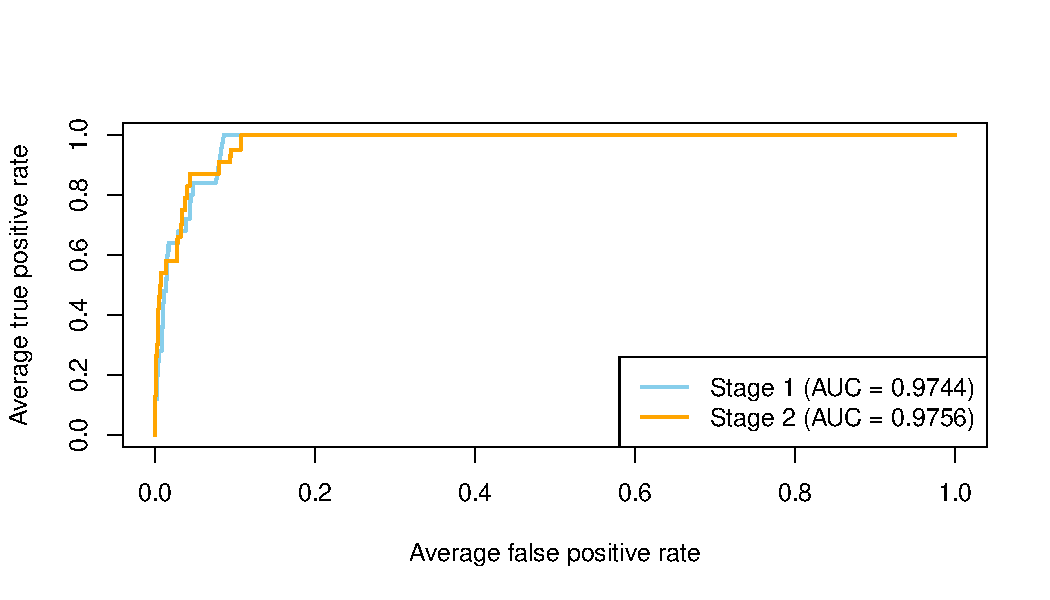
\includegraphics[width=\maxwidth]{figure/analyzeFI-1} \caption[Performance of DRaWR]{Performance of DRaWR}\label{fig:analyzeFI}
\end{figure}


\end{knitrout}
Figure 2 shows an ROC plot from the cross-validation produced by the
\texttt{analyze} method. 10\% of a query gene set is held out as a test set,
and the remaining gene set is used as query. Using the converged probability
distributions after the first stage and second stage RWR, ROC curves for two
stages are computed.

%------------------------------------------------------------
\subsection{Reporting}
%------------------------------------------------------------
The \texttt{analyze} method saves top-ranked AS events and pathways in the
\texttt{as.table} and \texttt{pathway.table} fields, respectively. If the
\texttt{samples} field contains information about sample conditions
(e.g. SF3B1 mutation), the results from gene set enrichment analysis are
included in the \texttt{pathway.table} field. The column \texttt{avg.rank}
is the average rank of gene nodes in the corresponding pathway. The last column
\texttt{neighborAS} is the number of AS event nodes in the final subnetwork
connected to the pathway.
\begin{knitrout}
\definecolor{shadecolor}{rgb}{0.969, 0.969, 0.969}\color{fgcolor}\begin{kframe}
\begin{alltt}
\hlcom{#Table of AS nodes in the final subnetwork}
\hlkwd{head}\hlstd{(GSE114922.ASpediaFI}\hlopt{$}\hlstd{as.table,} \hlnum{5}\hlstd{)}
\end{alltt}
\begin{verbatim}
                                                                                       node
3                                         VPS52:RI:chr6:33264900:33264782:33264497:33264374
4                 HMBS:SE:chr11:119092125:119092163:119092404:119092523:119092758:119092811
5 TUBGCP4:MXE:chr15:43400044:43400221:43401716:43403799:43404413:43404552:43405202:43405323
6                                 NAP1L4:A3SS:chr11:2976123:2976024:2972279:2972243:2972102
8   QTRT1:MXE:chr19:10707302:10707380:10707500:10707615:10712161:10712628:10712758:10712867
    prob
3 0.0041
4 0.0039
5 0.0038
6 0.0038
8 0.0037
\end{verbatim}
\begin{alltt}
\hlcom{#Table of GS nodes in the final subnetwork}
\hlkwd{head}\hlstd{(GSE114922.ASpediaFI}\hlopt{$}\hlstd{pathway.table,} \hlnum{5}\hlstd{)}
\end{alltt}
\begin{verbatim}
                      node   prob   pval   padj   ES  NES size avg.rank
1     HALLMARK_P53_PATHWAY 0.0089 0.1313 0.3759 0.24 1.22  121      709
2 HALLMARK_HEME_METABOLISM 0.0077 0.0001 0.0019 0.52 2.66  134      736
3      REACTOME_CELL_CYCLE 0.0037 0.0001 0.0019 0.28 1.51  323     1422
4      REACTOME_HEMOSTASIS 0.0028 0.6385 0.8923 0.17 0.95  257     1317
5            KEGG_LYSOSOME 0.0026 0.0211 0.0989 0.32 1.50   71      960
  neighborAS
1         58
2         59
3         59
4         59
5         59
\end{verbatim}
\end{kframe}
\end{knitrout}

%------------------------------------------------------------
\subsection{Visualization}
%------------------------------------------------------------
The \texttt{visualize} method enables visualization of AS events or pathways.
If the user provides an AS event nodes as input, it produces a plot
describing the AS event and a boxplot of PSI values. Note that the \texttt{gtf}
field must contain a \texttt{GRanges} object with genomic features extracted
from the GTF file. The genomic region around the AS event can be zoomed by
setting \texttt{zoom} to \texttt{TRUE}. Figure 3 illustrates the skipped exon of
HMBS, which has been shown to be associated with SF3B1 mutation in MDS.
\begin{knitrout}
\definecolor{shadecolor}{rgb}{0.969, 0.969, 0.969}\color{fgcolor}\begin{kframe}
\begin{alltt}
\hlcom{#Visualize AS event}
\hlstd{GSE114922.ASpediaFI}\hlopt{$}\hlkwd{visualize}\hlstd{(}\hlkwc{node} \hlstd{= GSE114922.ASpediaFI}\hlopt{$}\hlstd{as.table}\hlopt{$}\hlstd{node[}\hlnum{2}\hlstd{],}
                              \hlkwc{zoom} \hlstd{=} \hlnum{FALSE}\hlstd{)}
\end{alltt}
\end{kframe}\begin{figure}[H]
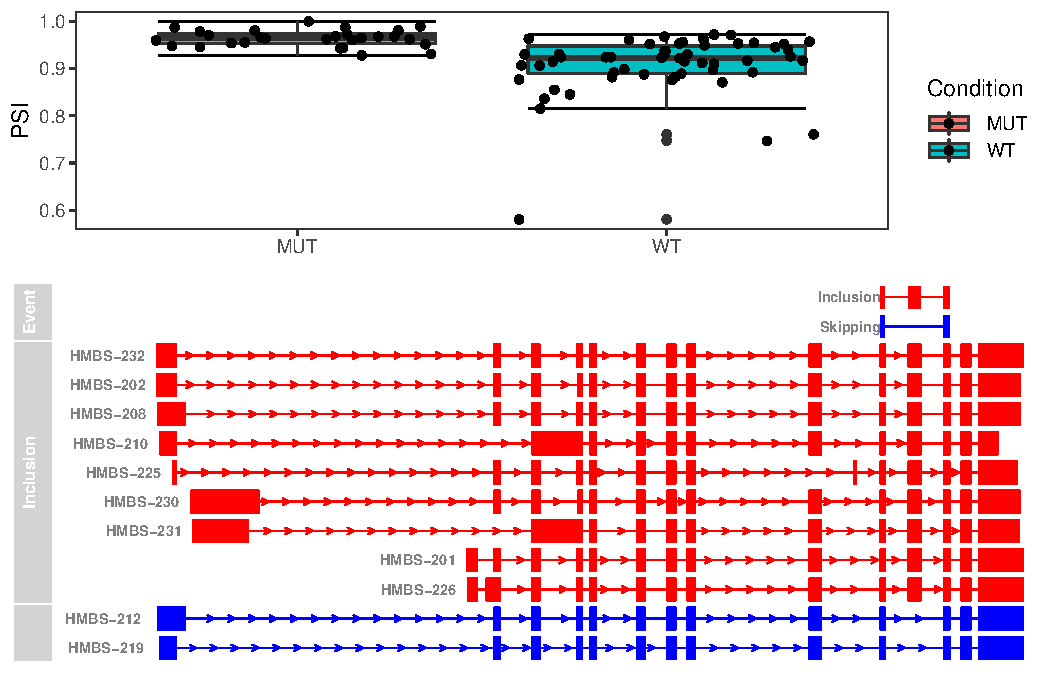
\includegraphics[width=\maxwidth]{figure/VizAS-1} \caption[AS event visualization]{AS event visualization}\label{fig:VizAS}
\end{figure}


\end{knitrout}
\pagebreak
If a pathway node is given, the \texttt{visualize} method shows a
subnetwork consisting of highly ranked gene nodes and AS event nodes connected
to the given pathway. The user can change the number of gene and AS event nodes
to be shown in the subnetwork by setting \texttt{n}. Figure 4 demonstrates the
subnetwork related to the hallmark pathway of heme metabolism which has also
been shown to be associated with SF3B1 mutation in MDS.
\begin{knitrout}
\definecolor{shadecolor}{rgb}{0.969, 0.969, 0.969}\color{fgcolor}\begin{kframe}
\begin{alltt}
\hlcom{#Visualize nework pertaining to specific pathway}
\hlstd{GSE114922.ASpediaFI}\hlopt{$}\hlkwd{visualize}\hlstd{(}\hlkwc{node} \hlstd{= GSE114922.ASpediaFI}\hlopt{$}\hlstd{pathway.table}\hlopt{$}\hlstd{node[}\hlnum{2}\hlstd{],}
                              \hlkwc{n} \hlstd{=} \hlnum{10}\hlstd{)}
\end{alltt}
\end{kframe}\begin{figure}[H]
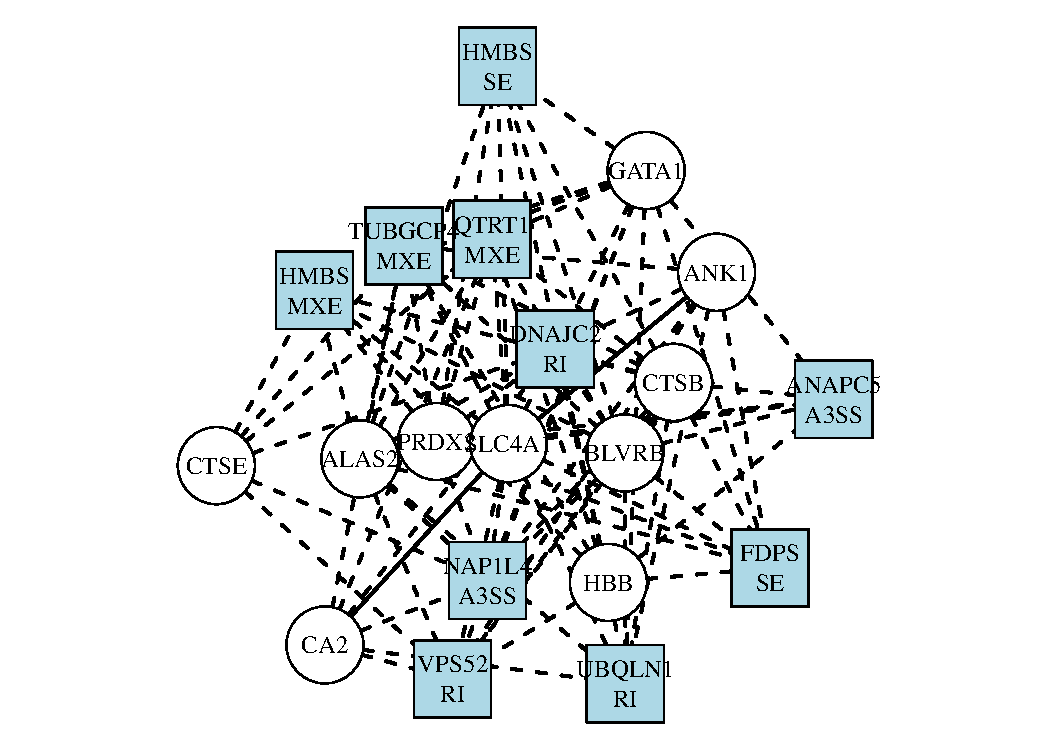
\includegraphics[width=\maxwidth]{figure/VizGS-1} \caption[Pathway visulization]{Pathway visulization}\label{fig:VizGS}
\end{figure}


\end{knitrout}

\renewcommand{\refname}{\section{References}}
\begin{thebibliography}{1}

\bibitem{gse114922}
Pellagatti, A. et al. (2018).
\newblock Impact of spliceosome mutations on RNA splicing in myelodysplasia:
dysregulated genes/pathways and clinical associations.
\newblock {\em Blood\/}, {\bf 132}, 1225--1240.

\bibitem{drawr}
Blatti, C. et al. (2016).
\newblock Characterizing gene sets using discriminative random walks with
restart on heterogeneous biological networks.
\newblock {\em Bioinformatics\/}, {\bf 32}, 2167--2175.

\end{thebibliography}


\end{document}
